\chapter{Einleitung}
\label{sec:Einleitung}

\section{CAN}
Controller Area Network (CAN) ist ein standardisiertes, robustes Fahrzeugbussystem, das für die Kommunikation zwischen verschiedenen Steuergeräten (ECUs) in Fahrzeugen und anderen industriellen Anwendungen konzipiert wurde. Es ermöglicht den zuverlässigen Datenaustausch mit hoher Fehlertoleranz und geringer Latenz, was besonders in Echtzeitanwendungen wichtig ist. CAN-Busse verwenden ein Nachrichtenbasiertes Protokoll, bei dem jede Nachricht eine eindeutige ID hat, die ihre Priorität bestimmt. Dieses System ist besonders nützlich bei der Diagnose von Netzwerkproblemen, da die Priorisierung von Nachrichten und Fehlererkennungsmechanismen die Fehlersuche erleichtern. Die physikalischen Aspekte des CAN-Busses, wie Abschlusswiderstände und die Verkabelung (CANL/CANH), sind ebenfalls entscheidend für die Netzwerkintegrität. Die Anpassungsfähigkeit hinsichtlich der Baudrate und die Unterstützung verschiedener Netzwerkstrukturen machen CAN vielseitig einsetzbar.\\

\section{Can-Datentelegram}
\begin{figure}[h]
    \centering
    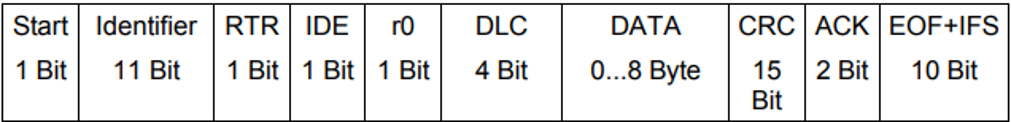
\includegraphics[width = 0.55\textwidth]{img/standard_datenframe.png}
    \caption{Standard Datentelegram}
    \label{fig: Standard Datentelegram}
\end{figure}
\begin{figure}[h]
    \centering
    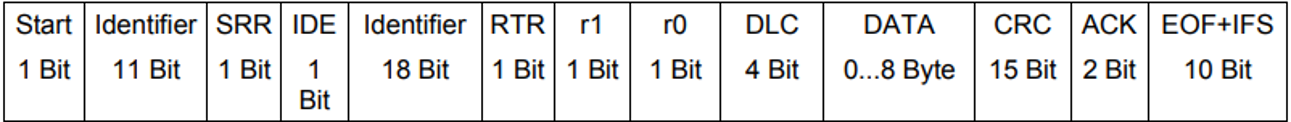
\includegraphics[width = 0.55\textwidth]{img/extended_datenframe.png}
    \caption{Extended Datentelegram}
    \label{fig: Extended Datentelegram}
\end{figure}

\noindent Ein CAN-Datentelegramm beginnt mit einem Startbit zur Synchronisation der kommunizierenden Geräte. Der Identifier gibt die Nachrichtenpriorität an und dient der Busarbitrierung, wobei das RTR-Bit zwischen einem Daten- und einem Datenanforderungstelegramm unterscheidet. IDE ist die Identifier Extension, die anzeigt, ob ein Standard- (11-Bit-Identifier siehe Abbildung \ref{fig: Standard Datentelegram}) oder ein Extended-Frame (29-Bit-Identifier siehe Abbildung \ref{fig: Extended Datentelegram}) verwendet wird. DATA enthält die eigentlichen Nutzdaten. CRC ist eine Prüfsumme zur Fehlererkennung. ACK signalisiert den korrekten Empfang der Nachricht. EOF und IFS kennzeichnen das Ende des Datentelegramms und den erforderlichen Abstand bis zum nächsten Frame. Im Extended Frame ersetzt das SRR-Bit das RTR-Bit des Standard Frames, und die DLC-Information gibt die Länge der Daten an.\\

\section{Anfordderungsanalyse}
\noindent Das "Can to Go"-System wird entwickelt, um Anwendern bei Problemen beim Aufbau eines CAN-Busses zu assistieren und zu diagnostizieren, wo genau die Schwierigkeiten liegen. Es dient als funktionssicherer CAN-Teilnehmer, der in der Lage ist, CAN-Nachrichten zuverlässig zu lesen und zu interpretieren. Kernmerkmale umfassen ein Anschlusskästchen mit SUB-D-Stecker und Status-LEDs, die den Betriebszustand des CAN-Busses anzeigen. Ein optionaler Abschlusswiderstand, der nach Bedarf zugeschaltet werden kann, sowie die Anpassungsfähigkeit der Baudrate gehören ebenfalls zu den wesentlichen Anforderungen. Darüber hinaus wird das System die CAN-Nachrichten und die zugehörigen Sender-IDs sichtbar machen.\\


\section{Endprodukt}


